\section{长情境教育部培训}\label{sec:long-context-training}

前面的部分在假设 MoE 层主导计算成本的情况下讨论了三堵墙（内存、通信和计算效率）。这一假设适用于序列长度为 4K--8K token 的典型训练任务，其中专家计算和全民通信是主要瓶颈。然而，推理模型的兴起（OpenAI o1、DeepSeek-R1 \cite{deepseekai2025deepseekr1}等）和基于强化学习的训练创造了一个新的领域：16K、64K 甚至更长的序列。在这些长度下，MoE 训练的性能特征发生了根本性的转变：注意力在计算中占主导地位，三堵墙的相对重要性也相应发生变化。本节研究长上下文训练如何重塑 MoE 模型的三堵墙，以及威震天核心如何应对新挑战。

\begin{figure}[ht]
    \centering
    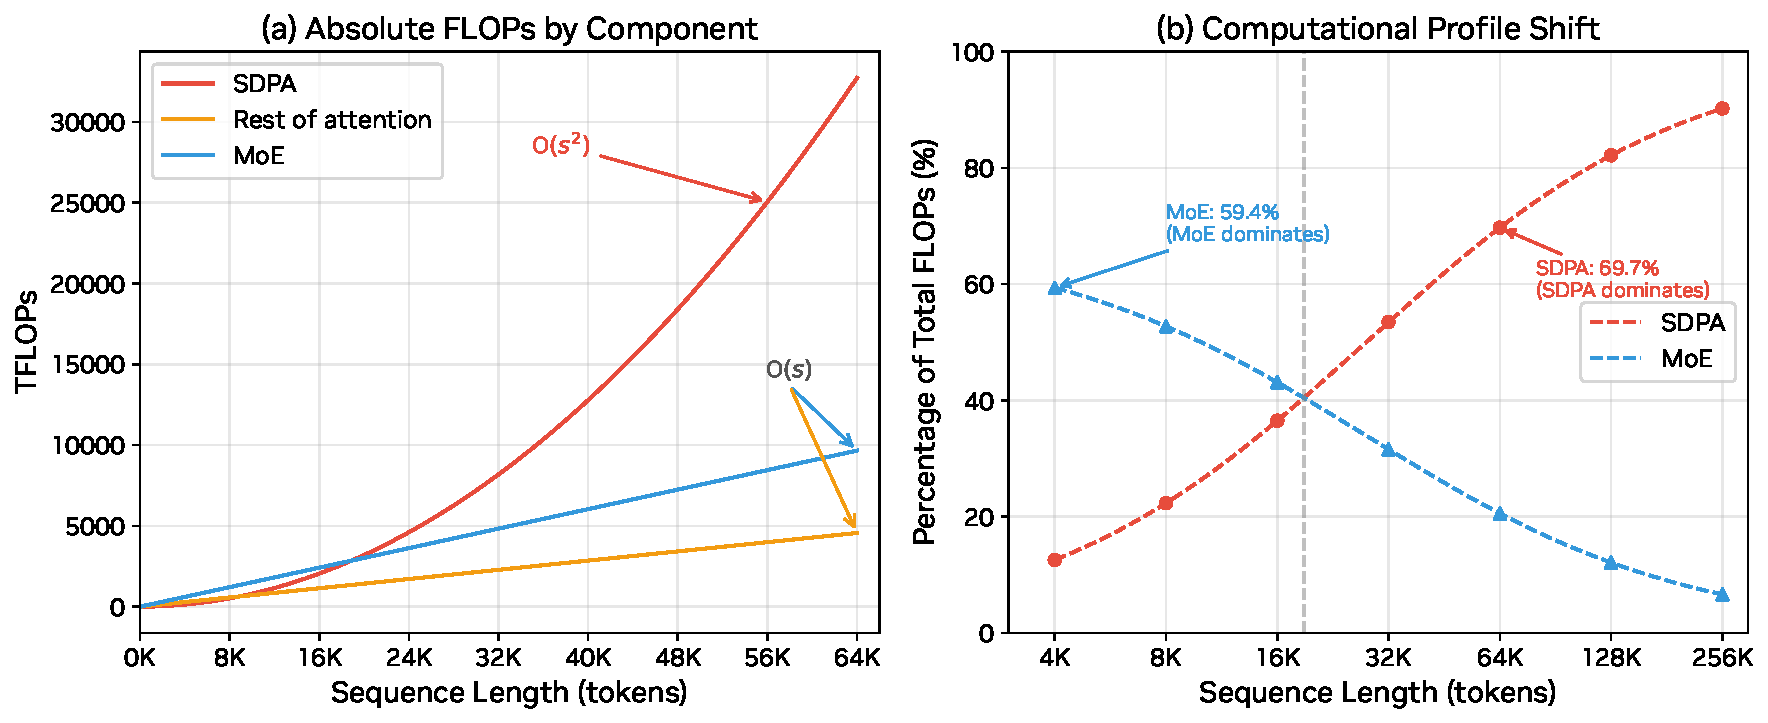
\includegraphics[width=1\linewidth]{figures/long_context_flops_ratio.pdf}
    \caption{SDPA展品 $O(s^2)$ 复杂性，而 MoE 和剩余的注意力操作表现出 $O(s)$ 复杂。因此，SDPA 在较长序列长度的计算中占主导地位。}
    \label{fig:long_context_flops_ratio}
\end{figure}

\subsection{当注意力占主导地位时：计算转变}

节中~\ref{key-features-optimizations}，我们确定 MoE 训练面临三个基本壁垒：内存、通信和计算效率。其中提出的优化（激活管理、调度程序优化、分组 GEMM 和 CUDA 图）针对 MoE 层在计算配置文件中占主导地位的场景。长情境训练从根本上改变了这一假设。关键的见解是 MoE 和注意力层之间不同的计算复杂性，如图所示 \figref{fig:long_context_flops_ratio}:
\begin{itemize}
    \item \textbf{MLP组件}：计算成本与序列长度成线性比例，表现出 $O(s)$ 复杂。
    \item \textbf{注意成分}：缩放点积注意力（SDPA）在计算成本中占主导地位，随序列长度呈二次方缩放，表现出 $O(s^2)$ 复杂。这种二次缩放激发了对有效注意力机制的广泛研究~\cite{beltagy2020longformer,zaheer2020bigbird}.
\end{itemize}

例如，对于 64K 代币，SDPA 消耗 69\% 的 FLOP 次数，相比之下只有 10--15\% 在短序列场景中。 \textbf{注意力在计算中占据主导地位。} 幸运的是，SDPA 在大多数 GPU 加速库（例如 FlashAttention）中都进行了高度优化 \cite{dao2022flashattention,dao2023flashattention2,shah2024flashattention3} 和 cuDNN（表~\ref{tab:sdpa-cudnn-perf}），所以SDPA不会成为性能瓶颈。因此，优化重点转向内存和通信：只要我们在不引入过多开销的情况下解决这两个挑战，就可以保持训练性能。

\begin{table}[ht]
\centering
\caption{DeepSeek-V3 的 cuDNN 中的 SDPA 性能。}
\label{tab:sdpa-cudnn-perf}
\begin{tabular}{cccc}
\toprule
\textbf{平台} & \textbf{序列长度} & \textbf{转发 TFLOPS} & \textbf{向后 TFLOPS} \\
\midrule
\multirow{2}{*}{Hopper}
 & 4096  & 553  & 422 \\
 & 16384 & 638  & 523 \\
\midrule
\multirow{2}{*}{Blackwell}
 & 4096  & 1324 & 1083 \\
 & 16384 & 1698 & 1298 \\
\bottomrule
\end{tabular}
\end{table}

\subsection{管理激活内存增长}

激活记忆随序列长度的增长是长上下文训练的主要挑战。为了解决这个强化的内存墙问题，我们应用了一组协同工作的技术，这些技术由大规模 MoE 工作负载提供信息，包括 DeepSeek-V3 \cite{deepseekai2025deepseekv3technicalreport} 和Qwen3 \cite{yang2025qwen3technicalreport}。这些技术扩展了第 1 节中介绍的内存优化原则~\ref{sec:memory-wall}.

\textbf{上下文并行和张量并行。}
将上下文并行 (CP) 和张量并行 (TP) 相结合可以跨设备分配激活内存，从而实现超出 GPU 容量的序列长度。关键原则是保持子序列长度（每个 CP/TP 分片的序列长度）大致恒定，通常为 4096 或 8192。 $\text{CP} \times \text{TP}$ 序列长度使每个设备的内存保持在基线水平附近。这使得工作负载类似于短上下文训练，除了 SDPA 和 TP/CP 特定的通信之外，因此大多数短上下文优化仍然适用。

\textbf{优化器 CPU 卸载。}
在大型模型中，优化器状态通常会消耗每个 GPU 数十 GB 的字节数。 CPU 卸载几乎可以完全回收这些内存，但代价是传输和主机端优化器开销。因此，选择是内存空间和吞吐量之间的权衡。对于 256 个 H100 GPU 上的 DeepSeek-V3，约为 50\% MFU和序列长度至少16K，最坏情况开销约为2\%。尽管确切的权衡取决于模型大小、序列长度和集群规模，但优化器 CPU 卸载对于长上下文训练通常是值得的。

\textbf{选择性重新计算。}
重新计算通过丢弃向前的中间激活并向后重新生成它们来计算内存。关键是基于内存与计算权衡的模块级选择性。在长上下文设置中，SDPA 在总计算中占主导地位，因此重新计算 SDPA（Megatron-Core 中的核心注意力重新计算）通常过于昂贵。相比之下，重新计算低成本组件（例如 MLP 相关模块）通常可以提供更好的净收益。对于 64K 序列长度的 DeepSeek-V3，SDPA 贡献高达 72\% 总计算量； recomputing it adds about 18\% 计算开销，导致大约 16\% 性能损失，仅节省 9 GB 内存。相反，重新计算非 SDPA 组件可在全局范围内节省 89.8 GB，同时对性能影响相当或更低。因此，我们建议禁用核心注意力重新计算并优先考虑其他模块的重新计算。

实际上，CP 和 TP 是长上下文记忆效率的主要机制。优化器 CPU 卸载和选择性重新计算可以提供额外的空间，尤其是在内存受限的平台上。这些技术可以很好地协同工作，并且可以根据需要进行组合。

\subsection{上下文并行与张量并行}

由于CP和TP是长上下文训练中最有效的两种策略，因此实际问题是当注意力主导计算时如何将它们结合起来。

CP和TP在长情境训练中都会减少激活记忆，但它们的沟通模式和记忆效果有所不同（图~\ref{fig:cp-comm-type}）。 CP 沿序列维度划分激活，并将激活内存减少为 $\text{CP}$。对于SDPA，CP有两种通信模式：点对点（P2P）和全对全（all-to-all）。 P2P CP以环形模式交换CP组内的KV缓存，与SDPA计算重叠~\cite{liu2023ringattention,brandon2023striped,jacobs2023deepspeedulysses}。 All-to-all CP 在 SDPA 之前将张量从序列分片形式转换为头分片形式，然后恢复序列分片形式。 TP 另外对线性权重进行了分片，减少了参数内存，但在线性层中引入了额外的集合。在 all-to-all CP 和 TP 中，SDPA 都在头分片张量上运行，这增加了每个分片子序列的长度并可以提高 SDPA 内核效率。

\begin{figure}[ht]
    \centering
    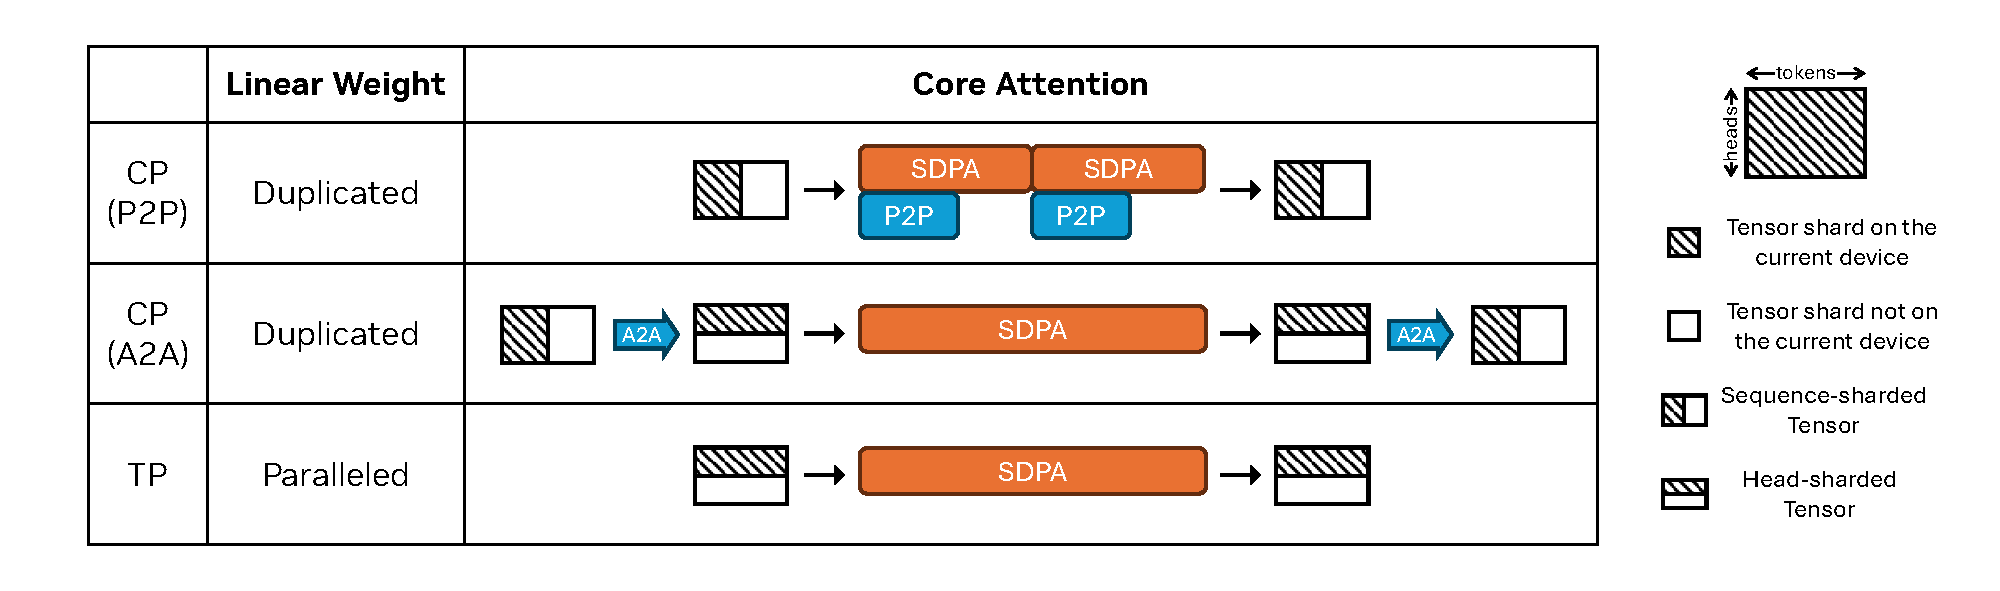
\includegraphics[width=1\linewidth]{figures/cp_comm_type.pdf}
    \caption{TP和两类CP的通信和计算模式。}
    \label{fig:cp-comm-type}
\end{figure}

在实际应用中，P2P CP是较为常见的CP模式。相对于TP，它的主要优点是通信与计算自然重叠，而TP通信往往更难隐藏。然而，TP 减少了密集的参数内存并可以提高 SDPA 效率。因此，TP 通常是节点内的首选，因为通信速度快且内存优势很强。在节点之间，P2P CP 通常变得更可取，因为 TP 通信开销会增加，而 P2P 重叠仍然有效。 All-to-all CP 介于两者之间：它避免了 P2P CP 使用的多步环交换，也避免了 TP 引入的线性权重分片开销。在实践中，当不希望进行环式交换且TP通信成本较高时，通常将All-to-all CP与TP结合起来进行节点内执行。

Megatron-Core 支持将两个 CP 后端组合为 \textbf{分层CP}，启用与 TP 的拓扑感知配对。一个实用的起点是在节点内部使用带有 TP 的全对所有 CP 来提高 SDPA 内核性能并减少参数内存，同时使用跨节点的 P2P CP 来保留通信计算重叠。这些是指导原则而不是硬性规则，但它们作为 TP/CP 调整的初始配置效果很好。

\subsection{用于可变长度训练的打包序列}\label{subsec:packed-sequence}

前面的小节研究了当序列长度增加时，三堵墙（内存、通信和计算效率）如何变化。这些分析假设每批内的序列长度固定。然而，实际训练场景，特别是强化学习和监督微调，通常涉及可变长度序列，这会带来额外的效率挑战。

传统的批处理需要将每个批次内的所有序列填充到最大长度，当序列长度变化很大时，会导致大量浪费~\cite{krell2021efficient}。例如，如果一个批次包含长度为 4K、8K 和 32K 令牌的序列，则所有序列都必须填充到 32K，从而浪费 $\sim$60\% 填充标记上的计算和内存。 This inefficiency compounds the memory and compute challenges discussed above.

为了解决这个问题，Megatron-LM 引入了 \textbf{打包序列} 在单个批次内处理可变长度序列，而不会造成填充浪费。此外，为了解决变长序列引起的DP不平衡和CP效率低下的问题，我们引入了 \textbf{动态上下文并行性（Dynamic-CP）}，它结合序列包装计划，在每个微批次的基础上自适应地选择有效的 CP 大小。

\subsubsection{打包序列支持}\label{subsec:packed_sequence_support}

Megatron-LM 支持打包序列，允许在单个批次内连接和处理多个可变长度序列，而无需序列间填充。这是通过 THD（总代币 $\times$ 头 $\times$ Dimension）张量格式，与传统的 SBHD（序列 $\times$ 批 $\times$ 头 $\times$ 尺寸）格式。 THD 将注意力张量表示为 \texttt{[total\_tokens, num\_heads, head\_dim]}，其中来自不同样本的序列沿着标记维度串联。

核心机制依赖于累积序列长度跟踪，它标记了打包张量中每个单独序列的开始和结束位置。这些参数通过注意力机制传播到 Transformer Engine 的融合内核，从而实现尊重序列边界的高效 SDPA 和 RoPE 操作。注意力计算使用累积序列长度来确保来自不同序列的查询和键不会相互关注，从而保持正确性，同时消除填充开销。

Megatron-LM 中的实现支持跨多个训练场景的打包序列：
\begin{itemize}
    \item \textbf{强化学习}：装箱算法将可变长度的轨迹分组到固定大小的箱中，从而最大限度地提高 GPU 利用率。
    \item \textbf{多式联运培训}：具有可变图像标记计数的视觉语言模型使用打包序列来处理来自不同数量的视觉块与文本标记组合的异构序列长度。
    \item \textbf{上下文并行集成}：当上下文并行性启用并满足填充要求时，系统会自动切换到 THD 格式，并提供填充和未填充的累积长度来处理通信对齐，同时保持计算效率。
\end{itemize}

打包序列支持的好处在长上下文场景中尤其明显。对于使用思维模型进行 RL 训练，序列长度可能从数百到数万个 token 不等，打包序列可以减少 40--60 的内存使用量\% 并将训练吞吐量提高1.5--2$\times$ 与传统的基于填充的方法相比。随着上下文长度超过 32K 令牌，这种效率增益变得越来越重要，否则填充浪费将主导内存消耗并显着减少有效批量大小。

\subsubsection{打包序列的动态上下文并行性}
\label{subsec:dynamic-cp}

虽然 THD 格式的打包序列消除了填充浪费，但它们并不能消除数据并行 (DP) 等级之间的计算不平衡。即使打包样本具有相同的总标记计数，由于点积注意力相对于子序列长度的二次复杂度，它们的注意力工作负载仍然可能有很大差异。例如， \Figref{fig:packing-sequences} 显示序列打包为相等的总长度，但作为 \Figref{fig:packing-sequence-imbalance} 表明，他们的计算工作负载差异很大。

这种 DP 不平衡会导致 GPU 在梯度同步点闲置，并可能进一步放大管道并行气泡。此外，当启用上下文并行性 (CP) 时，通常会选择静态 CP 大小来满足批次中最长打包样本的内存要求。因此，适合较少设备的较短封装样本仍被迫使用相同的 CP 大小，从而导致不必要的 CP 通信。在实践中，CP通信预计会被注意力计算隐藏；然而，在由许多短子序列组成的打包序列下，每个 CP 分片的计算可能不足以隐藏 CP 集合，特别是当 CP 跨越节点间链路时。我们将这种效应称为 CP 低效率。


    \begin{figure}[ht]
      \centering
      \begin{subfigure}[b]{0.48\textwidth}
        \centering
        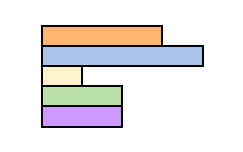
\includegraphics[width=0.8\textwidth]{figures/unpacked_sequence.pdf}
        \caption{解压序列。}
        \label{fig:unpacked-sequence}
      \end{subfigure}
      \hfill
      \begin{subfigure}[b]{0.48\textwidth}
        \centering
        \raisebox{0.8cm}{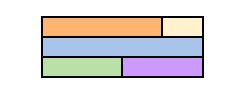
\includegraphics[width=0.8\textwidth]{figures/packed_sequence.pdf}}
        \caption{打包序列。}
        \label{fig:packed-sequence}
      \end{subfigure}
      \caption{未打包序列与打包序列。}
      \label{fig:packing-sequences}
    \end{figure}

    \begin{figure}[ht]
      \centering

        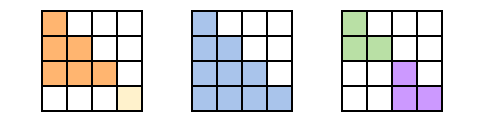
\includegraphics[width=0.8\textwidth]{figures/packed_sequence_imbalance.pdf}
        \caption{计算打包序列上因果注意力的不平衡。}
      \label{fig:packing-sequence-imbalance}
    \end{figure}

为了解决 DP 不平衡和 CP 效率低下的问题，我们引入了动态上下文并行（Dynamic-CP） \cite{nvidia_dynamiccp_blog}，它结合包装计划，在每个微批次的基础上自适应地选择有效的 CP 大小。关键的观察结果是，调整 CP 大小相对轻量级：它只改变令牌切片的划分方式以及注意力算子使用哪个 CP 通信组，而不需要任何参数重新分配或优化器状态迁移。因此，Dynamic-CP 为可变长度训练提供了一种实用的动态并行形式，并且框架开销最小。相关工作，包括ByteScale~\cite{ge2025bytescale} 和WLB-LLM~\cite{wang2025wlb}，解决类似的负载平衡挑战。


例如，考虑以下情况 \Figref{fig:input-sequences} 具有三个序列。我们假设只有两个 GPU 可用。如果我们采用标准 CP2 配置（即 DP=1，CP=2），工作负载将分两个微批次执行，如下所示 \Figref{fig:standard-cp}。在 microbatch-0 中，橙色序列足够长，必须在两个 GPU 之间进行分区。在 microbatch-1 中，打包的蓝色和绿色序列也分布在两个 GPU 上。然而，这对蓝色和绿色序列引入了不必要的分割，因为两个序列都可以适合单个 GPU 而不需要分区。

如图所示 \Figref{fig:dynamic-cp}，使用 Dynamic-CP，microbatch-0 中的橙色序列仍然需要 CP=2。在 microbatch-1 中，我们不再需要分割蓝色和绿色序列；相反，我们让它们每个都以 CP=1 独立运行。

    \begin{figure}[ht]
      \centering
      \begin{subfigure}[b]{0.19\textwidth}
        \centering
        \raisebox{0.8cm}{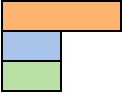
\includegraphics[width=0.8\textwidth]{figures/sequence_example.pdf}}
        \caption{输入序列。}
        \label{fig:input-sequences}
      \end{subfigure}
      \hfill
      \begin{subfigure}[b]{0.3\textwidth}
        \centering
        \makebox[\linewidth][c]{\raisebox{0.2cm}{\hspace*{-0.8cm}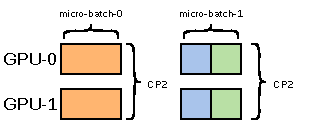
\includegraphics[width=1.4\textwidth]{figures/standard_cp.pdf}}}
        \caption{标准 CP2。}
        \label{fig:standard-cp}
      \end{subfigure}
        \hfill
      \begin{subfigure}[b]{0.3\textwidth}
        \centering
        \makebox[\linewidth][c]{\raisebox{0.2cm}{\hspace*{-0.8cm}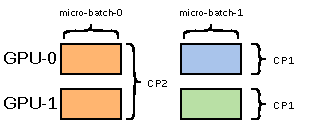
\includegraphics[width=1.4\textwidth]{figures/dynamic_cp.pdf}}}
        \caption{动态CP。}
        \label{fig:dynamic-cp}
      \end{subfigure}

      \caption{打包序列的动态上下文并行性。}
      \label{fig:dynamic-cp-example}
    \end{figure}


为了使每微批次 CP 大小调整在 Megatron-Core 中切实可行，Dynamic-CP 避免了任何昂贵的模型状态重新分配。相反，它将 CP 大小调整视为轻量级运行时选择：仅更改令牌切片的分区方式以及注意力操作符使用哪个 CP 通信组。具体来说，不是将每个等级绑定到单个静态构造的 \texttt{cp\_group}，框架在初始化期间为每个等级预先构建多个 CP 组，其中候选 \texttt{cp\_size} 范围从 1 到 \texttt{dp}$\times$\texttt{cp} （仅限于二人的权力）。在运行时，调度程序选择有效的 \texttt{cp\_size} 对于每个微批次和相应的预构建 \texttt{cp\_group}，启用动态 CP，而不会产生动态创建通信组的开销。

Dynamic-CP 专为 THD 布局而设计，其中可变长度序列在长度约束下打包，原始批次/序列维度折叠为令牌维度。一个直接的结果是微批次的数量不再是一个固定的数量 \texttt{global\_batch\_size} 和 \texttt{micro\_batch\_size};它可能会因迭代而变化，因为打包到每个微批次中的原始序列的数量不是恒定的。为了最大限度地减少对现有 Megatron-Core 管道调度程序的侵入性更改，Dynamic-CP 引入了轻量级 \texttt{data\_iterator\_wrapper} 围绕原来的 \texttt{data\_iterator}。对于每个全局批次，包装器 (i) 重新安排和打包序列以在 DP 等级之间创建平衡的工作负载，(ii) 选择有效的 \texttt{cp\_size} 对于每个微批次，以避免过度分片短包装样本，并且（iii）返回有效 \texttt{num\_microbatches} 对于当前迭代。由于通常只有排名的子集驱动 PP/VPP 下的调度决策，因此该框架广播动态调度元数据（包括 \texttt{num\_microbatches}, \texttt{max\_seqlen}， 和 \texttt{cu\_seqlens}）以确保跨管道阶段的一致执行。此外， \texttt{PackedSeqParams} 被扩展以携带所选的 \texttt{cp\_size} 和 \texttt{cp\_group};所有依赖于 CP 的组件（例如，位置嵌入和注意力）从以下位置检索 CP 配置： \texttt{PackedSeqParams} 而不是依赖全局静态 CP 变量。

给定 THD 中的可变长度序列，不同的样本贡献不同数量的有效标记。因此，损失是基于每个令牌计算的，以避免填充带来的偏差：
\begin{equation}
\mathcal{L} = \frac{\sum_{t\in \mathcal{V}} \ell_t}{|\mathcal{V}|},
\end{equation}
在哪里 $\mathcal{V}$ 表示打包表示中的有效（非填充）标记集。在规划方面，Dynamic-CP 求解器在 GPU 内存限制下共同确定打包和每微批次 CP 大小。由于注意力计算的规模大致为 $\mathcal{O}(S^2)$ 相对于子序列长度，而激活记忆规模更接近 $\mathcal{O}(S)$，很难同时平衡计算和内存。因此，Dynamic-CP 在面向工作负载和面向内存的决策之间交替：估计工作负载超过目标配额的微批次将被分配更大的容量 \texttt{cp\_size} 减少每列计算，之后内存成为主要约束，并通过选择计算量较少的样本来填充剩余容量，同时保留可行性。

最后，Dynamic-CP 的设计使运行时开销可以忽略不计。构建计划需要额外遍历全局批次以探测轻量级形状和序列长度元数据；通过在集群中分布探测并仅收集紧凑的元数据，可以减轻 I/O 压力。求解器本身异步运行（例如，在 \texttt{data\_sampler}）与训练迭代重叠。为了保持搜索空间的可管理性，穷举搜索被微批次计数上的一维网格搜索所取代，并受到约束，以便所有 DP 排名使用相同的 \texttt{num\_microbatches}。该计数是从 \texttt{PP}$\times$1 的小倍数 \texttt{PP}，捕获每微批次工作负载和管道气泡之间的权衡；在实践中，通过选择工作负载与微批次曲线上的“拐点”并仅探索其邻域，可以进一步缩小搜索范围。


总体而言，Dynamic-CP 通过以下方式补充打包序列训练：(i) 减少由 DP 不平衡引起的同步停顿；(ii) 防止无法从大 CP 大小中受益的微批次进行不必要的 CP 通信，从而提高长上下文可变长度训练的吞吐量。根据基准测试，Dynamic-CP 产生 35--60\% 在序列长度分布高度不平衡的现实场景（例如多模态训练）中实现端到端性能改进。 \footnote{探索 \href{https://github.com/NVIDIA/Megatron-LM/pull/2000}{公关\#2000} 和 \href{https://github.com/NVIDIA/Megatron-LM/pull/2959}{公关\#2959} 使用 Megatron-Core 优化开始训练具有可变长度序列的模型。}

\subsection{概括}

长上下文 MoE 训练代表了一种独特的优化机制，其中第 ~ 节的基本假设\ref{key-features-optimizations} 必须重新审视。虽然三堵墙（内存、通信和计算效率）仍然是基本障碍，但它们的相对重要性随着序列长度的增加而发生显着变化：

\begin{itemize}
    \item \textbf{计算转变}: 注意啦 $O(s^2)$ 复杂性取代 MoE 层成为主要的计算瓶颈，消耗 $>$ 69\% 失败次数 $>$ 64K 代币。 MoE重点优化的Section~\ref{sec:compute-wall} 仍然有价值，但不再解决主要瓶颈。
    
    \item \textbf{记忆墙强化}：激活内存随序列长度变化，需要第 4 节中的并行策略~\ref{parallelism-strategies} （特别是CP和TP）结合Section~的记忆技巧\ref{sec:memory-wall} （重新计算、卸载）以维持可行的内存占用。
    
    \item \textbf{沟通权衡}：CP 和 TP 之间的选择涉及通信开销、内存节省和 SDPA 计算效率之间的微妙权衡，这种平衡不同于第 3 节以 MoE 为中心的全面优化重点\ref{sec:comm-wall}.
\end{itemize}

通过结合上下文并行性、张量并行性、选择性重新计算和优化器卸载，Megatron-Core 可实现跨不同序列长度的高效训练。我们在 256 个 Hopper GPU 上以 256K 序列长度进行的实验证明了这一点：DeepSeek-V3 达到了 88\% 使用 TP、优化器 CPU 卸载和选择性重新计算的短上下文 MFU，而 Qwen3-235B-A22B 达到 129\% 其短上下文 MFU 具有 TP、CP 和选择性重新计算（后者超过 100\% 因为 SDPA 内核在主导较长序列的计算时效率很高）。打包序列和 Dynamic-CP 功能进一步将这些功能扩展到 RL 和 SFT 训练中的可变长度工作负载。


%==============================================================================
% SECTION 7: PRODUCTION Features
%==============================================================================

\section{生产特点}\label{sec:production-features}

前面的部分重点介绍了解决“三堵墙”问题的性能优化。然而，生产教育部培训还需要稳健性、灵活性和易用性。本节介绍满足这些操作要求的功能：确保稳定训练的负载平衡、共享和潜在的专家架构、用于灵活部署的分布式检查点、升级以使用现有的密集模型，以及与多令牌预测等高级训练范例的集成。

\subsection{负载均衡和令牌丢弃}

MoE 模型中的动态路由可能会导致严重的工作负载不平衡，某些专家会比其他专家获得更多的代币。这会导致计算效率低下、内存瓶颈和硬件利用率下降。我们通过两种协调机制来应对这些挑战：负载平衡和令牌丢弃。

\textbf{负载平衡。}
\Figref{fig:load-balancing-strategies} 说明了威震天核心 MoE 中可用的负载平衡策略。 
我们提供多种策略来鼓励统一的代币分配。主要方法采用 \textbf{辅助损失}~\cite{lepikhin2020gshard,fedus2022switchtransformersscalingtrillion}，一个可微的惩罚项，不鼓励将所有令牌路由到一小部分专家。我们也支持 \textbf{专家选择路由}~\cite{zhou2022mixtureofexpertsexpertchoicerouting}，它将平衡路由制定为最优传输问题，并且 \textbf{辅助无损耗平衡} 通过可学习的专家偏差术语~\cite{wang2024auxiliarylossfreeloadbalancingstrategy} 根据历史负载动态调整路由决策。

\textbf{代币掉落。}
我们支持两种具有不同容量管理策略的调度策略。在 \textit{无滴模式} （默认），所有路由令牌的处理都没有容量限制，从而以每个专家工作负载的可变性为代价最大化模型表达能力。在 \textit{可放置模式}，执行明确的专家容量限制~\cite{lepikhin2020gshard,fedus2022switchtransformersscalingtrillion}：当分配给专家的令牌超出其容量时，多余的令牌将被丢弃并通过剩余连接绕过。这提供了可预测的内存范围，在路由器初始化不良时的早期训练期间非常有用。

\textbf{静态形状的 Pad-to-Max。}
可放置模式还可以 \textit{填充到最大} 功能，它将所有专家输入填充到相同的容量限制。这将 MoE 固有的动态每个专家令牌计数转换为静态形状，从而实现诸如 CUDA 图形之类的优化（第 ~\ref{sec:cuda-graphs}）需要在迭代中固定张量维度。

\begin{figure}[ht]
    \centering
    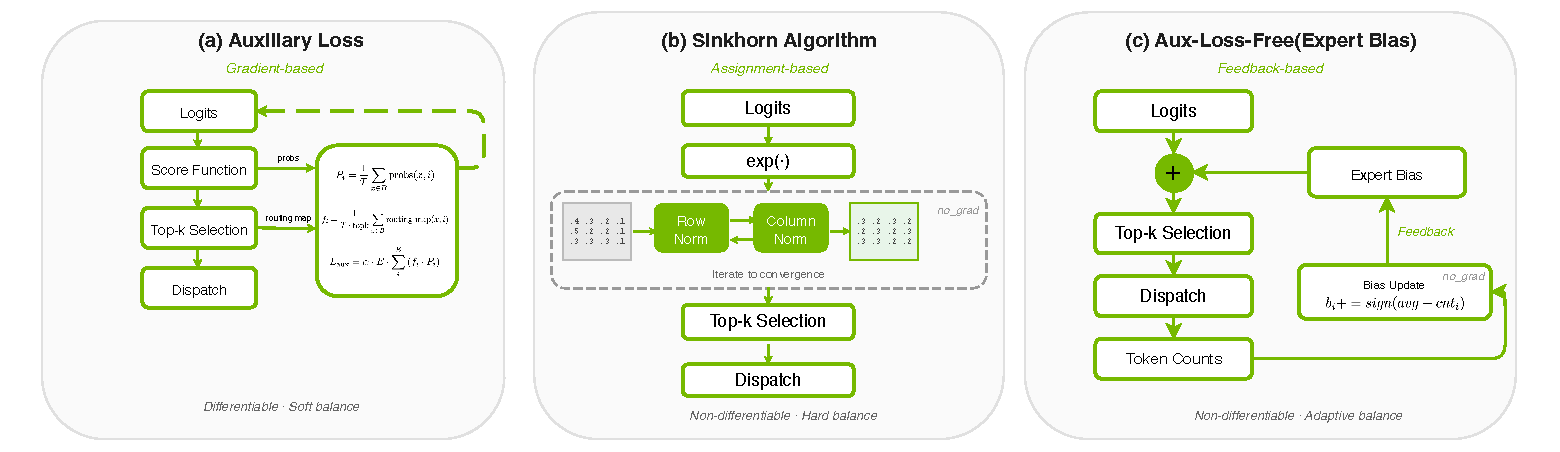
\includegraphics[width=\textwidth]{figures/load-balancing-strategies.drawio.pdf}
    \caption{Megatron-Core MoE 中的负载平衡策略。}
    \label{fig:load-balancing-strategies}
\end{figure}%

\subsection{共享专家}

一些 MoE 架构（DeepSeek-V2/V3 \cite{deepseekai2024deepseekv2strongeconomicalefficient,deepseekai2025deepseekv3technicalreport}, 琪文 \cite{qwen2025qwen25technicalreport}）包括一个共享专家，无论路由如何，都可以处理所有令牌，从而为所有令牌提供一致的基线容量（\figref{fig:shared-expert-architecture}）。当启用重叠时（\texttt{-{}-moe-shared-expert-overlap}），共享专家计算与所有通信和路由专家计算并行运行，将其延迟隐藏在调度-计算-组合管道后面。

\begin{figure}[ht]
    \centering
    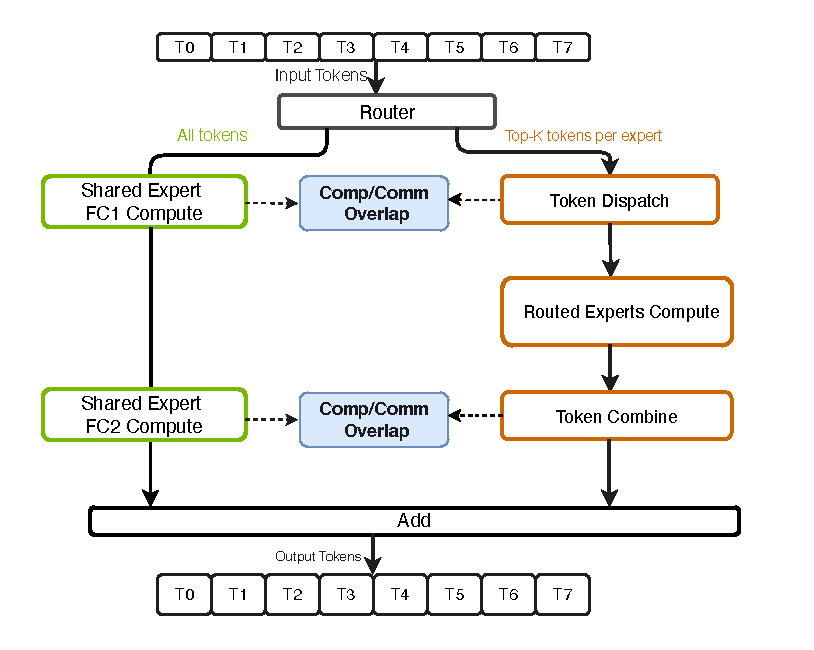
\includegraphics[width=0.7\textwidth]{figures/shared-expert-architecture.drawio.pdf}
    \caption{Megatron-Core MoE 中的共享专家架构。共享专家流程 \emph{全部} 令牌，而路由专家仅处理分配给他们的令牌。启用重叠后，共享专家计算与令牌调度/组合通信并行运行，隐藏其延迟。}
    \label{fig:shared-expert-architecture}
\end{figure}

\subsection{潜在的教育部}\label{sec:latent-moe}

在标准 MoE 中，all2all 通信在完全隐藏维度上调度令牌 \(d\)，每个专家都由权重矩阵参数化 \(\mathbb{R}^{m \times d}\) 和 \(\mathbb{R}^{d \times m}\)。潜伏MoE~\cite{elango2026latentmoe} 通过插入共享下投影来降低这两种成本 \(W_\downarrow \in \mathbb{R}^{\ell \times d}\) 在调度和向上投影之前 \(W_\uparrow \in \mathbb{R}^{d \times \ell}\) 合并后，其中 \(\ell < d\) 是潜在维度。路由仍然在完全隐藏的维度上运行，以保持路由质量；每个被路由的专家完全在压缩的潜在空间中运行；共享专家仍处于维度 \(d\)。层输出变为：
\[
\text{output}(\mathbf{x}) = W_\uparrow \cdot \Bigl(\sum_{i \in \mathcal{T}_{K,E}} p_i \, E_i(W_\downarrow \cdot \mathbf{x};\, \ell)\Bigr) + \sum_{j} E_j^{\text{shared}}(\mathbf{x};\, d).
\]

压缩比 \(\alpha = d / \ell\) 将 all2all 通信量减少一倍 \(\alpha\) （代币在维度上发送 \(\ell\) 而不是 \(d\)）和每个专家的权重大小相同的因子（专家矩阵从 \(\mathbb{R}^{m \times d}\) 到 \(\mathbb{R}^{m \times \ell}\)）。埃兰戈等人~\cite{elango2026latentmoe} 定义两种利用这些节省的方法。在 \(\ell\text{-MoE}_{\text{eff}}\), 专家总数 \(E\) 缩放比例为 \(\alpha\) 而顶部-\(K\) 不变，以降低的推理成本保持基线精度。在 \(\ell\text{-MoE}_{\text{acc}}\) （推荐），两者 \(E\) 和顶部-\(K\) 缩放比例为 \(\alpha\)，它将推理成本恢复到标准 MoE 水平，但呈指数级扩展专家选择的组合空间（\(\binom{\alpha E}{\alpha K} \geq \binom{E}{K}^{\alpha}\)），以等成本产生更高的精度。在高达 95B 参数的范围内， \(\ell\text{-MoE}_{\text{acc}}\) 在每 FLOP 和每个参数的准确性方面始终优于标准 MoE。该架构已被 NVIDIA 的 Nemotron-3 Super 和 Ultra 型号采用。

\textbf{执行。}
LatentMoE 通过启用 \texttt{-{}-moe-latent-size}，其中设置 \(\ell\)。这 \texttt{MoELayer} 实例化两个 \texttt{TELinear} 预测： \texttt{fc1\_latent\_proj} （下投影在 \texttt{preprocess} 步骤，在路由之后但在分派之前）和 \texttt{fc2\_latent\_proj} （上投影在 \texttt{postprocess} 步骤，合并后）。专家后端（\texttt{TEGroupedMLP}, \texttt{SequentialMLP}）自动调整它们的输入和输出尺寸 \(\ell\).

